\chapter{Future Research and Other Projects}
\label{ch:future}

\section{Improvements to eCryptfs Boundary Mode}
\label{sec:future}

The illustration which concludes the previous chapter, of Alice securely reminding herself to send flowers, may be contrived, but it
is a pattern that can be used to secure locally stored data for nearly any application. The scenario was tested on an actual phone,
running actual code, and it works, but there is a lot that still needs to be done before this could be used in any practical sense.
As Dan Kaminsky once tweeted, ``The game is not to secure you, or me. Security for security people is just a self licking ice cream
cone.'' What follows are a few ideas for future work.

\subsection{Configurable Application Security}
There is, as it stands, no way to configure which applications will have their boundary keys cleared when the device sleeps. 
Each application \texttt{uid} and package name must be hardcoded, which is only meant to demonstrate that the 
boundary keys do function. A user interface would be beneficial. This interface could tie to the ``manage applications'' menu and
should provide an easy, intuitive way for the user to select which applications will be protected while the device is locked.

\subsection{Securely Handle Keys}
The primary achievement of eCryptfs boundary mode is that it forces an attacker to use live memory analysis to recover keys. That is
considerably more difficult than simply copying the data off the device. Already, live forensic techniques are being developed for
the Android platform \cite{dmd}, but they require considerably more skill to execute than post-mortem techniques. The next
step on the privacy side of this arms race is to prevent all access to secured application data on a live system, even in the face of
live memory analysis. The primary hurdle is that very little of the code involved was
designed to withstand memory-based attacks. Android does \emph{not} handle the unlock password or the key material derived from that
password securely. Table \ref{tab:badhandling} shows the code responsible for retrieving the unlock password from the lock screen
and running it through \texttt{checkPassword}. The password is stored in a standard Java string, which is \emph{not} a secure
way to store strings in memory.
\begin{table}[htpb]
\lstinputlisting{tables/unlock.java}
\caption{The wrong way to handle passwords in java}
\label{tab:badhandling}
\end{table}
The Sun recommended method for storing passwords in memory is to use a \texttt{char} array, not a \texttt{String} object
\cite{securejava}. This is because \texttt{java.lang.String} objects are immutable. They cannot be zeroed out after usage. Arrays of
characters can, however, be zeroed. It is not conceptually difficult to audit the password handling routines in Android for insecure
handling, but it is time consuming and tedious. Validating that the password was being handled securely would require developing a
tool for recovering password keys from memory. Joe Sylve's work could be used \cite{dmd} for validation, but the tools accompanying his paper 
had not yet been released at the time of writing.

\subsection{Utilize \texttt{ecryptfsd} and encrypt SD card}
As a demonstration of what could be done, boundary keys are currently being calculated directly in the kernel. This allowed for
rapid development, but may not be the wisest place. Instead of hooking the passphrase keying mode of
eCryptfs, an additional keying mode with a different header format could be developed. This mode could call out to
\texttt{ecryptfsd} for boundary key calculation. Pushing this portion out into userspace would provide a great deal more flexibility
regarding the criteria to use for generating boundary keys. If someone wanted to use the GID\footnote{Group ID} instead of the UID
for a particular eCryptfs volume, for example, that could be easily configured. The ability to use the GID would be
advantageous because it would afford encryption of external storage with eCryptfs. The problem now is that all SD card files are
owned by \texttt{system}. Clearing the boundary key for \texttt{system} is not an option, as it would result in instability of the
device. The SD card files have a group owner of \texttt{sdcard\_rw}, though, so if the boundary key were calculated using the
GID, then it could be cleared. More generally, calling out to \texttt{ecryptfsd} would allow for arbitrary logic when
boundary keys are being created.

\section{Data Contraception}
Up to this point, it has been assumed that the goal was to prevent access to some piece of data on the device.  Once a forensic
artifact has touched disk, and especially if any wear-leveling is happening, it can be very difficult to remove.  Completely
wiping a partition is deemed by many to be forensically sound, but is a difficult and cumbersome task on the Android platform.  Data can
be securely deleted from a YAFFS2 filesystem, but only with considerable difficulty due to the necessity of keeping track of every
chunk that a piece of data was ever written to. If a hardware ``flash translation layer'' is being used for wear-leveling, as is the
case for most newer phones, then it may be nearly impossible to remove artifacts once they are written.  Encrypting the whole mess
is a great start, but relying solely on encryption still leaves the chance that if the key is exposed, then historical forensic
artifacts can be recovered.

Data ``contraception,'' is more reliable, if more difficult to implement and validate.  Data contraception is a term first
introduced by The Grucq, who pioneered the field of anti-forensics \cite{defiling}.  The idea is that forensic analysis cannot find
that which has not been created.  The cost is significant modification to the underlying architecture of whatever application or
operating system is creating the forensic artifacts of concern.  The most obvious and descriptive example from the Android platform
is browser history.  The ability to obtain browser history from any platform is one of the most basic forensic techniques, and it
remains central to any Android analysis.  This is the principle of ``Incognito Mode" in the Chrome desktop browser and the Android
browser in versions 3.x and later. When incognito mode is enabled, all browsing history remains in memory and never touches disk. A
Linux live CD is capable of doing the same thing, but with an entire operating system instead of just a browser.

As of yet, there has been little exploration of the possibility of a memory-only Android device, where no data is ever written. 


\section{Validating Privacy Tools}
All forensic tools must be validated before they are considered to be of any value. Privacy tools should be held to the same
standard, but there is very little literature on validating privacy tools. This section outlines what it might mean to validate a
privacy tool and gives an example. Validating privacy tools is one of the most important steps the security community could take
toward enhancing the privacy of users.

If a given forensic tool exists that can retrieve a known artifact, the corresponding privacy tool should prevent the retrieval of
that artifact. For purposes of this section, the forensic tool retrieving data is called the reference tool. When developing tests
for privacy tools, the test is only meaningful in the context of this reference tool. A tool which prevents the recovery of browser
history, for example, presupposes that a reference tool which recovers browser history is available and can itself successfully pass
traditional forensic validation, to an extent appropriate to the situation.

Brian Carrier has provided a clear and thoughtful expose \cite{Carrier2003} on the requirements of forensic tools.  Though his paper
is primarily a legal argument for using open-source acquisition and extraction tools, the insights he provides along the way have
direct counterparts in the privacy arena and can be used as general guidelines here.  Every forensic tool must pass, in a repeatable
fashion, tests which demonstrate that it does retrieve the information the tool purports to retrieve.  If a forensic tool claims to
recover browser history, for example, it may be tested by salting a device with known browser history and attempting to retrieve the
data with the tool.  As noted by Carrier, The NIST Computer Forensic Tool Testing (CFTT) group publishes a wide variety of test
methodologies and the results of those tests.  While CFTT tests provide good reference material, and provide detailed tests for
classic forensic techniques such as disk imaging, none of their published documents provide a specific testing methodology for
modern smart-phones. 

While a reference tool may be developed specifically for the purpose of developing a privacy tool, doing so increases the risk of
insufficient or biased testing.  Any reference tool developed purely for the purpose of testing a privacy tool is suspect, as the
tool had not been previously published nor accepted by the forensics community.  Whenever possible, privacy tools should be
validated against forensic techniques developed by someone other than the author of the privacy tool.  This can be difficult as the
field of Android forensics is relatively new, and there was until very recently little literature on how Android forensics is
performed. The field is growing at an astonishing rate, however, and tools are becoming easier to find.

\subsubsection{Why Validation is Necessary: CyanogenMod Incognito Mode}

CyanogenMod is a popular after-market build of Android that is compatible with many Android devices.  While the primary developer of
CyanogenMod is Steve Kondik, who goes by the handle Cyanogen, it is a community project; notably, several members of the
influential \emph{xda-developers} forum have contributed code.  Based on the Android Open Source Project, CyanogenMod offers a
number of enhancements that are not in the core Android code, though some features such as USB tethering were later introduced.
Users are driven to CyanogenMod because it offers a high quality alternative to the version of Android packaged for their
phone.  Often CyanogenMod runs the latest version of Android long before an official build is released by the manufacturer, making
CyanogenMod very attractive for people with older phones, even if it requires rooting the phone to install.  CyanogenMod has become
such an important Android distribution that some phone manufacturers have begun actively endorsing it, and Samsung even hired Steve
Kondik.

One of the features of CyanogenMod that is actively promoted is incognito mode. The incognito mode in CyanogenMod 7 is not, however,
the incognito mode that is included with Ice Cream Sandwich, as CyanogenMod 7 is based on Gingerbread. According to the CyanogenMod
web site, incognito mode prevents browsing and download history from being saved, in addition to deleting all cookies.
\footnote{http://www.cyanogenmod.com/features/incognito-mode} It does actually do these things, and the browser history removal has
been validated.  Unfortunately, the discovery of a very important artifact, cache, is not being protected against. Failure to remove
browser cache leaves browser history discoverable.

\subsubsection{Browser History Validation}

The browser history on an Android device is stored in the \texttt{browser.db} database.  In a vanilla distribution of Android , this
database is stored in the \texttt{/data/data/com.android.browser/databases} directory.  Oddly enough, the browser history is stored
in the bookmarks table.  The screen clipping in figure \ref{fig:bookmarkschema} shows the bookmarks table as it is seen in SQLite
browser.  Bookmarks and page visits are stored nearly identically by the Android browser, with the bookmark integer being set to 0
if it is a normal page visit and to 1 if the URL is a bookmark.  Bookmarks also commonly store thumbnails of the saved page.
\begin{figure}[htpb]
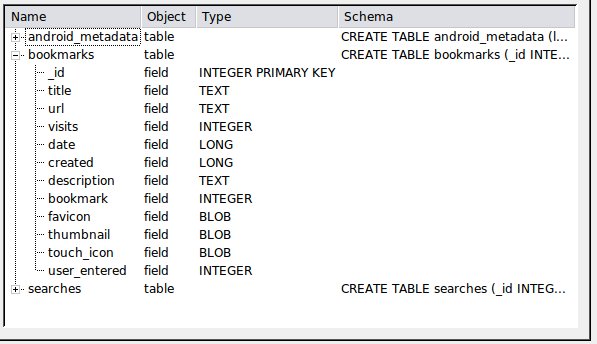
\includegraphics[scale=0.75]{BookmarksSchema.png}
\caption{Bookmarks Table Schema in SQLite browser}
\label{fig:bookmarkschema}
\end{figure}

Nearly every person who has ever used a browser is now aware that browsers keep a list of visited sites.  Browsers, however, also
come with a mechanism to erase this history, but few are aware of the ineffectiveness of deleting browser history.  Many an
investigation has turned on a forensic analyst's ability to recover deleted browser history records.  Moreover, any system which
requires the user to remember to clear their browser history is bound to fail.  The most obvious solution is to simply disable
browser history.  It may or may not be more desirable to keep a temporary, memory-only browser history history during the browser
session, but disabling is more straightforward and more secure.  The pertinent code is in the browser provider, and the function in
table \ref{tab:incognito} disables all inserts into the history database.

\begin{table}[htpb]
\lstinputlisting{tables/incognito.java}
\caption{Basic incognito mode: bypass history insert}
\label{tab:incognito}
\end{table}

It is a less than subtle, but effective, hack.  By blowing away the \texttt{updateVisitedHistory} method and immediately returning,
the user is guaranteed that the browser history database will never be written to.  This is, in essence, what the ``Incognito Mode"
in the popular CyanogenMod ROM does. The above method was tested side-by-side with CyanogenMod 7.

\begin{enumerate}
\item \url{www.slashdot.org} was chosen as the site for salting the device
\item The browser history was visually inspected in the browser itself
\item The browser database was pulled with \texttt{adb}
\item A case-insensitive substring search of the entire data partition was performed with the Linux \texttt{strings} utility
\item A \texttt{nanddump} was carved for deleted SQLite records containing browser history
\item The absence of references to the salt site was confirmed
\item The native Android browser was opened, and only \url{www.slashdot.org} was visited
\item The browser history was pulled from the device in the same manner as above
\item It was confirmed that there are references to the salt site
\item Repeated for device running CyanogenMod 7 (visiting \url{www.slashdot.org} with incognito mode enabled) and analyzed acquired data
\item Repeated for device running the custom history bypass and analyzed acquired data
\end{enumerate}

As expected, after the data partition is wiped there is no information in the browser history.  The browser database itself is
missing until the browser is launched for the first time.  After the salt site is visited, it is clearly visible in the browser
history available on the device and in the browser database as a unique record.  When incognito mode is enabled in CyanogenMod,
neither method produces results indicative of a visit to the salt site.


\subsubsection{Browser Cache Validation}
The Android browser cache is a particularly interesting forensic artifact.  The browser cache is implemented within the webkit
framework, rather than the browser application.  There are, therefore, no content providers in the Android API that expose the
browser cache, making it difficult to erase from the user interface, yet the cache is written as normal files to the data partition
and indexed in a SQLite database.  These files provide a wealth of forensic information about browsing history, second only to the
browser history itself, and often the data is of more use than the browser history as it contains the actual content viewed.
Because the files are written to disk, even if the application data is cleared, the cached files can usually be recovered,
especially if a log-structured filesystem such as YAFFS2 is being used.  Because the browser cache is not implemented within the
browser application itself, some trivial attempts to implement incognito mode in the Android browser have overlooked the browser
cache.  This test will do a three-way comparison: the results of a custom method completely disabling cache are contrasted with
stock Gingerbread and CyanogenMod 7.

In order to validate that the browser cache is prevented from being written to disk, attempts to retrieve the cache will be made using
\texttt{adb}.  It has been established elsewhere that once data is written to flash, there is a high probability of recovery even if
the data is deleted \cite{naval}. The database \texttt{/data/data/com.android.browser/databases/webviewCache.db} contains the index of the
browser cache, and \texttt{/data/data/com.android.browser/cache/webviewCache} and subdirectories contains the actual cache files. 

\begin{enumerate}
\item \url{www.slashdot.org} was  the chosen site for salting the device
\item The browser cache in the above locations was pulled from an empty device
\item It was confirmed that there are no records in the SQLite database referring to the salt site
\item It was confirmed that there are no files in \texttt{/data/data/com.android.browser/cache/webviewCache} or subdirectories containing a case-insensitive substring match for the word 'slashdot'
\item The native Android browser was opened, and only \url{www.slashdot.org} was visited
\item The browser cache was pulled from the device
\item It was confirmed that records in the SQLite database and files indicating a visit to \url{www.slashdot.org} existed
\item Repeated for device running CyanogenMod 7 (visiting \url{www.slashdot.org} with incognito mode enabled) and analyzed acquired data
\item Repeated for device with custom cache bypass and analyzed acquired data
\end{enumerate}

On the empty device no databases and no cache files were found in the \texttt{/data/data/com.android.browser} directory.  As
expected, the logical acquisition process was successful in retrieving cached data after the browser has been opened and
\url{www.slashdot.org} visited.  Once the browser had been opened on a device running stock Android, the \texttt{webviewCache.db}
database was populated with data from the default page that loads. 

After visiting \url{www.slashdot.org} and pulling the database with \texttt{adb}, a \texttt{SELECT * FROM cache WHERE url LIKE
'\%slashdot\%'} listed several records.  Similarly, a \texttt{grep -ri 'slashdot' webviewCache} showed a significant amount of
\url{www.slashdot.org} data in the cache files.  This validates that the forensic tool is able to find references to a particular
site in the web cache.

In CyanogenMod 7, the \texttt{webviewCache.db} records and the cache files created in
\texttt{/data/data/com.android.browser/cache/webviewCache} directory are indistinguishable from stock Android.  Completely disabling
cache, in contrast, entirely prevents the creation of cache files and entries into webviewCache.db.  In fact, webviewCache.db is
never created, as it is initialized as a temporary database.  After visiting \url{www.slashdot.org} in the native Android browser, a
logical acquisition using \texttt{adb} recovered no cache data from \texttt{/data/data/com.android.browser}.  While the incognito
mode built into CyanogenMod 7 passed the browser history artifact test, it does not pass the browser cache artifact test. This is
because the browser cache is implemented by webkit, and the CyanogenMod 7 incognito mode operates entirely within the browser
application. 

\section{Other Projects}

Chapter \ref{ch:fde} introduced full-disk encryption in WhisperCore, but there are other noteworthy privacy-oriented projects for Android. 

\subsubsection{Orbot and Orweb}

Orbot is an implementation of Tor for Android. Tor stands for ``the onion router,'' and is an implementation of onion routing,
which was patented by the United States Navy in the late 1990s.  Onion routing works by randomly routing traffic through a series of
relays, encrypting the traffic in a series of layers, one for each relay (like an onion). Routers in the Tor network know which
router a packet came from, and which router is next, but nothing else. The entrance and exit routers can see the content of the
message, but are unaware of the destination and source, respectively. This allows for relatively anonymous internet connections, and
has been used worldwide to access the internet in countries which censor the internet. Orbot works on a non-rooted Android phone,
but is much easier to configure if the device has root access available. Because users often betray their identity through their
browser, even when using Tor, the Tor project ships a configured version of Firefox that is tailored for privacy. The Android
equivalent of the Tor browser is Orweb.


\subsubsection{TextSecure}

Whisper Systems, which was acquired by Twitter in late 2011, produced a number of other great projects that were included with
WhisperCore. RedPhone was one of these. It provided an Android implementation of encrypted voice traffic, utilizing ZRTP.
Unfortunately the RedPhone service was shutdown after Whisper Systems was acquired by Twitter. TextSecure, however, was
open-sourced. TextSecure provides encrypted SMS messaging for Android using the Off-the-Record (OTR) protocol. OTR is wonderfully
clever.It gets its name from ``off the record'' journalism sourcing, where the source remains anonymous. In OTR, in addition to
traditional encryption, two features are included: perfect forward secrecy and deniability. Perfect forward secrecy uses
temporary session keys that are not reproducible if the master key is compromised. So, if Alice sends a message to Bob, and at a
later date the NSA compromises either Alice or Bob's key (or both), the conversation cannot be recreated.  Deniability refers to the
ability of the participants in a conversation to deny that the conversation ever happened. In OTR, the participants are able to
authenticate each other during the conversation, but a third-party cannot prove that the conversation occurred. To be clear, it can
be established that \emph{a} conversation occurred between the two participants, but the contents of that conversation cannot be
proven to be authentic \cite{otr}.


\section{Summary}

If privacy tools are to be developed that are capable of securing data against state-of-the-art forensic techniques, then there is
still a great deal of work that needs to be done. The field of mobile forensics is progressing at a rate that far exceeds the
field of mobile privacy. An easy-to-use form of disk encryption that is resistant to live memory analysis is desperately needed.  If
securing a device requires intimate knowledge of that device's internals, then in practice it will never be secured. This paper has
taken steps toward building an encryption scheme for Android that is resistant to logical analysis and could, with minimal
development, be resistant to live memory analysis. This encryption method in particular, and all privacy tools in general, need to
be rigorously and thoroughly validated. If there are bugs in them, the privacy community needs to find them before an attacker does.
